\chapter{Additional Data}
\section{Control Variate Results}
Detailed results for \acl{CV} presented in \autoref{ch:cvinsrns} are given in \autoref{tab:eff1}, \autoref{tab:eff2}, and \autoref{tab:eff3}.
\begin{figure}[htb]
    \centering
    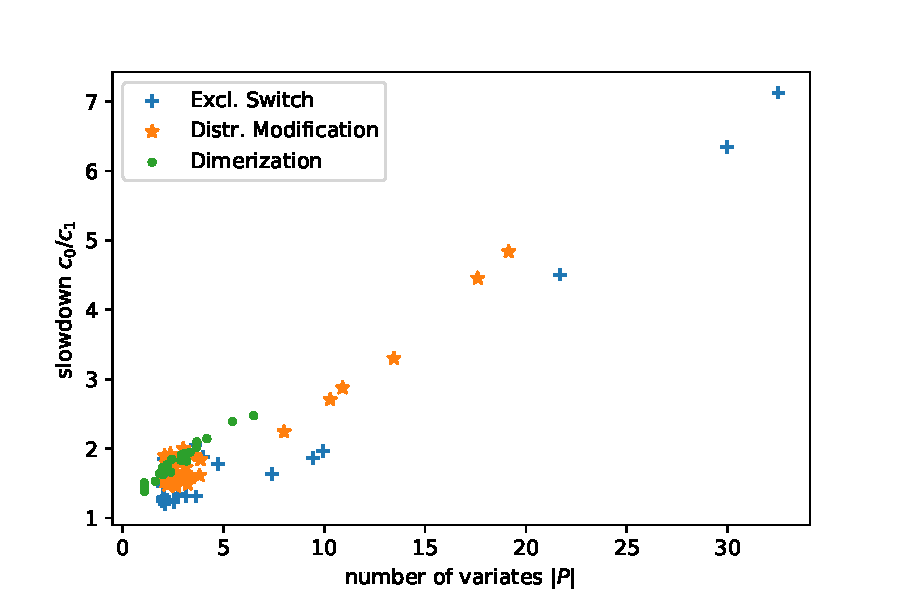
\includegraphics[width=0.8\textwidth]{gfx/cv_slowdown.pdf}
    \caption{The slowdown $c_0/c_1$ v.\ the number of control variates $|P|$.}
\end{figure}
%\section{Linear Control Variates}
\begin{table}[htb]
    \centering
	\resizebox{\textwidth}{!}{
\begin{tabular}{l@{\hskip 12pt}l@{\hskip 12pt}l@{\hskip 12pt}r@{\hskip 12pt}r@{\hskip 12pt}r@{\hskip 12pt}r}
\toprule
	$n_{\max}$ &   $n_{\lambda}$ & $\phi$ & $1-\frac{\sigma_1^2}{\sigma_0^2}$ &  slowdown &  efficiency &$\lvert P\rvert$ \\\midrule
	\num{1}& $10$ &$\phi_{sq}$ &  $0.807184$ &  $1.227471$ &    $4.239255$ &   $2.536479$ \\
            &    &$\phi_{c}$ &  $0.880285$ &  $1.633530$ &    $5.135205$ &   $7.411732$ \\
            &    &$\phi_{q}$ &  $0.849082$ &  $1.312416$ &    $5.067770$ &   $3.639250$ \\
            &    & $\phi_{\ell}$ &  $0.783459$ &  $1.195821$ &    $3.874778$ &   $2.090101$ \\\cmidrule{2-7}
            & $20$ &$\phi_{sq}$ &  $0.856593$ &  $1.263340$ &    $5.539683$ &   $2.206154$ \\
            &    &$\phi_{c}$ &  $0.910480$ &  $1.864405$ &    $6.011256$ &   $9.441336$ \\
            &    &$\phi_{q}$ &  $0.867987$ &  $1.317958$ &    $5.765884$ &   $3.140806$ \\
            &    & $\phi_{\ell}$ &  $0.825518$ &  $1.243075$ &    $4.627662$ &   $1.981143$ \\\cmidrule{2-7}
            & $30$ &$\phi_{sq}$ &  $0.869165$ &  $1.298893$ &    $5.905196$ &   $2.059415$ \\
            &    &$\phi_{c}$ &  $0.921019$ &  $1.966191$ &    $6.461331$ &   $9.928998$ \\
            &    &$\phi_{q}$ &  $0.876822$ &  $1.340409$ &    $6.079876$ &   $2.762449$ \\
            &    & $\phi_{\ell}$ &  $0.843288$ &  $1.288925$ &    $4.968796$ &   $1.983174$ \\\midrule
	\num{2} & $10$ &$\phi_{sq}$ &  $0.811956$ &  $1.505521$ &    $3.544783$ &   $2.323999$ \\
            &    &$\phi_{c}$ &  $0.916866$ &  $4.507566$ &    $2.681363$ &  $21.692390$ \\
            &    &$\phi_{q}$ &  $0.868874$ &  $1.776190$ &    $4.309354$ &   $4.739893$ \\
            &    & $\phi_{\ell}$ &  $0.795802$ &  $1.466579$ &    $3.353046$ &   $2.016196$ \\\cmidrule{2-7}
            & $20$ &$\phi_{sq}$ &  $0.832562$ &  $1.657484$ &    $3.617313$ &   $2.085711$ \\
            &    &$\phi_{c}$ &  $0.934280$ &  $6.348223$ &    $2.406431$ &  $29.976320$ \\
            &    &$\phi_{q}$ &  $0.878944$ &  $1.879341$ &    $4.416281$ &   $3.990881$ \\
            &    & $\phi_{\ell}$ &  $0.837922$ &  $1.647329$ &    $3.759896$ &   $1.978017$ \\\cmidrule{2-7}
            & $30$ &$\phi_{sq}$ &  $0.829427$ &  $1.844766$ &    $3.190308$ &   $2.043201$ \\
            &    &$\phi_{c}$ &  $0.947324$ &  $7.130628$ &    $2.673225$ &  $32.513670$ \\
            &    &$\phi_{q}$ &  $0.878830$ &  $2.053317$ &    $4.034987$ &   $3.611746$ \\
            &    & $\phi_{\ell}$ &  $0.824936$ &  $1.838879$ &    $3.118728$ &   $1.978836$ \\
\bottomrule
\end{tabular}}
    \caption[Variance reduction results for up to second order moments]{Variance reduction results for up to second order moments with parameters $n_{\max}=2$, $n=\num{10000}$, $d=100$, $k_{\min}=3$. Exclusive switch.}
    \label{tab:eff1}
\end{table}

\begin{table}[htb]
    \centering
	\resizebox{\textwidth}{!}{
\begin{tabular}{l@{\hskip 12pt}l@{\hskip 12pt}l@{\hskip 12pt}r@{\hskip 12pt}r@{\hskip 12pt}r@{\hskip 12pt}r}
\toprule
	$n_{\max}$ &   $n_{\lambda}$ & $\phi$ & $1-\frac{\sigma_1^2}{\sigma_0^2}$ &  slowdown &  efficiency &$\lvert P\rvert$ \\\midrule
$1$ & $10$ &$\phi_{sq}$ &  $0.619560$ &  $1.488483$ &    $1.770218$ &   $3.232575$ \\
            &    &$\phi_{c}$ &  $0.700255$ &  $2.241695$ &    $1.492171$ &   $8.008607$ \\
            &    &$\phi_{q}$ &  $0.643550$ &  $1.613001$ &    $1.743500$ &   $3.817641$ \\
            &    & $\phi_{\ell}$ &  $0.596650$ &  $1.459405$ &    $1.703170$ &   $2.657000$ \\\cmidrule{2-7}
            & $20$ &$\phi_{sq}$ &  $0.697414$ &  $1.519425$ &    $2.181687$ &   $2.631677$ \\
            &    &$\phi_{c}$ &  $0.713445$ &  $2.706546$ &    $1.292838$ &  $10.295856$ \\
            &    &$\phi_{q}$ &  $0.697654$ &  $1.585313$ &    $2.092817$ &   $3.398235$ \\
            &    & $\phi_{\ell}$ &  $0.695846$ &  $1.473976$ &    $2.235418$ &   $2.226530$ \\\cmidrule{2-7}
            & $30$ &$\phi_{sq}$ &  $0.712941$ &  $1.543068$ &    $2.263644$ &   $2.378037$ \\
            &    &$\phi_{c}$ &  $0.721354$ &  $2.874249$ &    $1.252541$ &  $10.910880$ \\
            &    &$\phi_{q}$ &  $0.711877$ &  $1.607712$ &    $2.164485$ &   $2.979704$ \\
            &    & $\phi_{\ell}$ &  $0.669963$ &  $1.522184$ &    $1.996300$ &   $2.085473$ \\\midrule
$2$ & $10$ &$\phi_{sq}$ &  $0.619450$ &  $1.734737$ &    $1.519168$ &   $3.148184$ \\
            &    &$\phi_{c}$ &  $0.665361$ &  $3.301159$ &    $0.909443$ &  $13.456259$ \\
            &    &$\phi_{q}$ &  $0.680592$ &  $1.840457$ &    $1.705876$ &   $3.864240$ \\
            &    &$\phi_{\ell}$ &  $0.612674$ &  $1.662962$ &    $1.556868$ &   $2.659592$ \\\cmidrule{2-7}
            & $20$ &$\phi_{sq}$ &  $0.684789$ &  $1.811408$ &    $1.755652$ &   $2.687379$ \\
            &    &$\phi_{c}$ &  $0.689835$ &  $4.455005$ &    $0.726640$ &  $17.609554$ \\
            &    &$\phi_{q}$ &  $0.687665$ &  $1.901258$ &    $1.688449$ &   $3.413595$ \\
            &    &$\phi_{\ell}$ &  $0.651262$ &  $1.770238$ &    $1.623924$ &   $2.266729$ \\\cmidrule{2-7}
            & $30$ &$\phi_{sq}$ &  $0.690602$ &  $1.922217$ &    $1.686011$ &   $2.375455$ \\
            &    &$\phi_{c}$ &  $0.649191$ &  $4.837419$ &    $0.591701$ &  $19.145054$ \\
            &    &$\phi_{q}$ &  $0.701253$ &  $2.001179$ &    $1.677062$ &   $3.007525$ \\
            &    &$\phi_{\ell}$ &  $0.639123$ &  $1.894074$ &    $1.467403$ &   $2.086275$ \\
\bottomrule
\end{tabular}}
    \caption[Variance reduction results for up to second order moments]{Variance reduction results for up to second order moments with parameters $n_{\max}=2$, $n=\num{10000}$, $d=100$, $k_{\min}=3$. Distributive modification.}
    \label{tab:eff2}
\end{table}

\begin{table}[htb]
    \centering
\begin{tabular}{l@{\hskip 12pt}l@{\hskip 12pt}l@{\hskip 12pt}r@{\hskip 12pt}r@{\hskip 12pt}r@{\hskip 12pt}r}
\toprule
	$n_{\max}$ &   $n_{\lambda}$ & $\phi$ & $1-\frac{\sigma_1^2}{\sigma_0^2}$ &  slowdown &  efficiency &$\lvert P\rvert$ \\\midrule
	\num{1} & $10$ &$\phi_{sq}$ &  $0.881641$ &  $1.530137$ &    $5.558692$ &   $1.621917$ \\
            &    &$\phi_{c}$ &  $0.965224$ &  $1.945588$ &   $14.859417$ &   $3.338501$ \\
            &    &$\phi_{q}$ &  $0.916445$ &  $1.625232$ &    $7.409904$ &   $1.997045$ \\
            &    & $\phi_{\ell}$ &  $0.868288$ &  $1.380344$ &    $5.529745$ &   $1.081152$ \\\cmidrule{2-7}
            & $20$ &$\phi_{sq}$ &  $0.941153$ &  $1.637272$ &   $10.437978$ &   $1.842971$ \\
            &    &$\phi_{c}$ &  $0.964204$ &  $1.907999$ &   $14.747328$ &   $2.915082$ \\
            &    &$\phi_{q}$ &  $0.947984$ &  $1.747519$ &   $11.072422$ &   $2.227250$ \\
            &    & $\phi_{\ell}$ &  $0.931030$ &  $1.433401$ &   $10.169570$ &   $1.088572$ \\\cmidrule{2-7}
            & $30$ &$\phi_{sq}$ &  $0.959517$ &  $1.723449$ &   $14.404936$ &   $1.972426$ \\
            &    &$\phi_{c}$ &  $0.962514$ &  $1.770936$ &   $15.142156$ &   $2.216103$ \\
            &    &$\phi_{q}$ &  $0.966216$ &  $1.847441$ &   $16.117387$ &   $2.446661$ \\
            &    & $\phi_{\ell}$ &  $0.945724$ &  $1.456432$ &   $12.710196$ &   $1.084188$ \\\midrule
	\num{2} & $10$ &$\phi_{sq}$ &  $0.905254$ &  $1.659799$ &    $6.402491$ &   $2.388472$ \\
            &    &$\phi_{c}$ &  $0.987526$ &  $2.474939$ &   $33.074955$ &   $6.501180$ \\
            &    &$\phi_{q}$ &  $0.923063$ &  $1.822654$ &    $7.195544$ &   $3.179257$ \\
            &    & $\phi_{\ell}$ &  $0.878232$ &  $1.415909$ &    $5.830248$ &   $1.092264$ \\\cmidrule{2-7}
            & $20$ &$\phi_{sq}$ &  $0.949038$ &  $1.831995$ &   $10.797164$ &   $2.890898$ \\
            &    &$\phi_{c}$ &  $0.985710$ &  $2.391457$ &   $29.704344$ &   $5.450299$ \\
            &    &$\phi_{q}$ &  $0.968076$ &  $2.021487$ &   $15.662368$ &   $3.681229$ \\
            &    & $\phi_{\ell}$ &  $0.925413$ &  $1.449386$ &    $9.298961$ &   $1.072761$ \\\cmidrule{2-7}
            & $30$ &$\phi_{sq}$ &  $0.964855$ &  $1.924268$ &   $14.911787$ &   $3.026275$ \\
            &    &$\phi_{c}$ &  $0.981507$ &  $2.144089$ &   $25.520987$ &   $4.179125$ \\
            &    &$\phi_{q}$ &  $0.973902$ &  $2.095985$ &   $18.507746$ &   $3.685851$ \\
            &    & $\phi_{\ell}$ &  $0.948349$ &  $1.507425$ &   $12.904707$ &   $1.074538$ \\
\bottomrule
\end{tabular}
    \caption[Variance reduction results for up to second order moments]{Variance reduction results for up to second order moments with parameters $n_{\max}=2$, $n=\num{10000}$, $d=100$, $k_{\min}=3$. Dimerization.}
    \label{tab:eff3}
\end{table}

\section{Aggregation for Stationary Distributions}
Experimental results of aggregation for stationary distribution approximation presented in \autoref{ch:statagg} are given in \autoref{tab:par_bd} and \autoref{tab:excl_switch}.
\begin{table}[h]
    \centering
	{\scriptsize
\begin{adjustbox}{angle=90}
    \begin{tabular}{l l rrrrrrrr}
        \toprule
        \multicolumn{2}{c}{} & \multicolumn{8}{c}{iteration $i$} \\\cmidrule(lr){3-10}
	    $\epsilon$ & & \num{1} & \num{2} & \num{3} & \num{4} & \num{5} & \num{6} & \num{7} & \num{8}  \\
         \midrule
	    \multirow{3}*{\e{1}{-1}} 
	     & $|\mathcal{S}^{(i)}|$ & \num{4900} & \num{28} & \num{52} & \num{112} & \num{232} & \num{472} & \num{960} & \num{1932} \\
	    & tot.\ error & \num{1.91} & \num{1.84} & \num{1.73} & \num{1.55} & \num{1.29} & \e{9.35}{-1} & \e{4.88}{-1} & \e{3.54}{-2}\\
	    & max.\ error & \e{3.15}{-3} & \e{3.13}{-3} & \e{3.08}{-3} & \e{2.98}{-3} & \e{2.77}{-3} & \e{2.38}{-3} & \e{1.57}{-3} & \e{6.04}{-5} \\
         \midrule
	    \multirow{3}*{\e{1}{-2}}
	    & $|\mathcal{S}^{(i)}|$ & \num{4900} & \num{52} & \num{104} & \num{208} & \num{464} & \num{988} & \num{2008} & \num{4052} \\
	     & tot.\ error & \num{1.91} & \num{1.84} & \num{1.73} & \num{1.56} & \num{1.30} & \e{9.46}{-1} & \e{5.01}{-1} & \e{6.22}{-4}\\
		    & max.\ error & \e{3.15}{-3} & \e{3.13}{-3} & \e{3.08}{-3} & \e{2.98}{-3} & \e{2.78}{-3} & \e{2.39}{-3} & \e{1.59}{-3} & \e{8.33}{-7}\\
         \midrule
	    \multirow{3}*{\e{1}{-3}}
	    & $|\mathcal{S}^{(i)}|$ & \num{4900} & \num{84} & \num{152} & \num{300} & \num{652} & \num{1440} & \num{2996} & \num{6068} \\
	    & tot.\ error & \num{1.91} & \num{1.83} & \num{1.73} & \num{1.56} & \num{1.30} & \e{9.46}{-1} & \e{5.01}{-1} & \e{9.83}{-6}\\
		     & max.\ error & \e{3.15}{-3} & \e{3.13}{-3} & \e{3.08}{-3} & \e{2.98}{-3} & \e{2.78}{-3} & \e{2.39}{-3} & \e{1.59}{-3} & \e{1.14}{-8}\\
	             \midrule
	    \multirow{3}*{\e{1}{-4}}
	    & $|\mathcal{S}^{(i)}|$ & \num{4900} & \num{116} & \num{212} & \num{400} & \num{848} & \num{1872} & \num{3960} & \num{8060} \\
	     & tot.\ error & \num{1.91} & \num{1.83} & \num{1.73} & \num{1.56} & \num{1.30} & \e{9.46}{-1} & \e{5.01}{-1} & \e{9.83}{-6}\\
	    & max.\ error & \e{3.15}{-3} & \e{3.13}{-3} & \e{3.08}{-3} & \e{2.98}{-3} & \e{2.78}{-3} & \e{2.39}{-3} & \e{1.59}{-3} & \e{1.83}{-10}\\
	             \bottomrule
    \end{tabular}
\end{adjustbox}
	}
    \caption[Stationary distribution approximation results for \autoref{model:par_bd}]{Detailed results for Model~\ref{model:par_bd}. The errors are computed wrt.\ the reference Poissonian product. The total absolute error and the maximum absolute errors are given.}
    \label{tab:par_bd}
\end{table}
\begin{table}
    \centering
	{\scriptsize
	\begin{adjustbox}{angle=270}
    \begin{tabular}{L{8mm} l rrrrrrrr}
        \toprule
        \multicolumn{2}{c}{} & \multicolumn{8}{c}{iteration $i$} \\\cmidrule(lr){3-10}
	    $\epsilon$ & & \num{1} & \num{2} & \num{3} & \num{4} & \num{5} & \num{6} & \num{7} & \num{8}  \\
         \midrule
	    \multirow{3}*{\e{1}{-1}}
	    & $|\mathcal{S}^{(i)}|$ & \num{11907} & \num{20} & \num{32} & \num{60} & \num{140} & \num{340} & \num{840} & \num{2116} \\
	    & tot.\ error $\leq$ & \e{1.86}{0} & \e{1.85}{0} & \e{1.45}{0} & \e{1.18}{0} & \e{9.31}{-1} & \e{6.41}{-1} & \e{4.67}{-1} & \e{4.89}{-1} \\
	    & max.\ error $\leq$ & \e{1.63}{-3} & 1.63e-3 & \e{1.55}{-3} & \e{1.40}{-3} & \e{1.22}{-3} & \e{9.36}{-4} & \e{8.40}{-4} & \e{1.40}{-3} \\
         \midrule
	    \multirow{3}*{\e{1}{-2}}
	    & $|\mathcal{S}^{(i)}|$ & \num{11907} & \num{48} & \num{112} & \num{148} & \num{300} & \num{720} & \num{1892} & \num{5156} \\
	    & tot.\ error $\leq$ & \e{1.86}{0} & \e{1.84}{0} & \e{1.44}{0} & \e{1.21}{0} & \e{9.56}{-1} & \e{6.65}{-1} & \e{3.41}{-1} & \e{3.31}{-2} \\
	    & max.\ error $\leq$ & \e{1.63}{-3} & \e{1.62}{-3} & \e{1.53}{-3} & \e{1.39}{-3} & \e{1.20}{-3} & \e{9.59}{-4} & \e{5.86}{-4} & \e{5.37}{-5} \\
         \midrule
	    \multirow{3}*{\e{1}{-3}}
	    & $|\mathcal{S}^{(i)}|$ & \num{11907} & \num{84} & \num{192} & \num{244} & \num{488} & \num{1084} & \num{2692} & \num{7152} \\
	    & tot.\ error $\leq$ & \e{1.86}{0} & \e{1.83}{0} & \e{1.46}{0} & \e{1.22}{0} & \e{9.63}{-1} & \e{6.67}{-1} & \e{3.37}{-1} & \e{8.01}{-4} \\
	    & max.\ error $\leq$ & \e{1.63}{-3} & \e{2.95}{-2} & \e{1.54}{-3} & \e{1.39}{-3} & \e{1.20}{-3} & \e{9.51}{-4} & \e{5.79}{-4} & \e{1.09}{-6} \\
         \midrule
	    \multirow{3}*{\e{1}{-4}}
	    & $|\mathcal{S}^{(i)}|$ & \num{11907} & \num{124} & \num{324} & \num{352} & \num{672} & \num{1436} & \num{3408} & \num{8864} \\
	    & tot.\ error $\leq$ & \e{1.86}{0} & \e{1.83}{0} & \e{1.46}{0} & \e{1.22}{0} & \e{9.63}{-1} & \e{6.67}{-1} & \e{3.37}{-1} & \e{1.12}{-5} \\
	    & max.\ error $\leq$ & \e{1.63}{-3} & \e{3.19}{-2} & \e{1.54}{-3} & \e{1.39}{-3} & \e{1.20}{-3} & \e{9.51}{-4} & \e{5.79}{-4} & \e{1.28}{-8} \\
         \bottomrule
    \end{tabular}
\end{adjustbox}
	}
	\caption[Stationary distribution approximation results for \autoref{model:excl_switch}]{Detailed results for \autoref{model:excl_switch}. Upper bounds on the total absolute error and the maximum absolute error are given. The worst-case errors are computed wrt.\ the reference Geobound solution with $\epsilon_{\ell}=\e{1}{-2}$.}
    \label{tab:excl_switch}
\end{table}
